\section{Additional Experimental Results}
\label{app:additional-experimental-results}

\begin{figure}[h]
    \centering
    \begin{subfigure}[t]{0.31\textwidth}
        \centering
        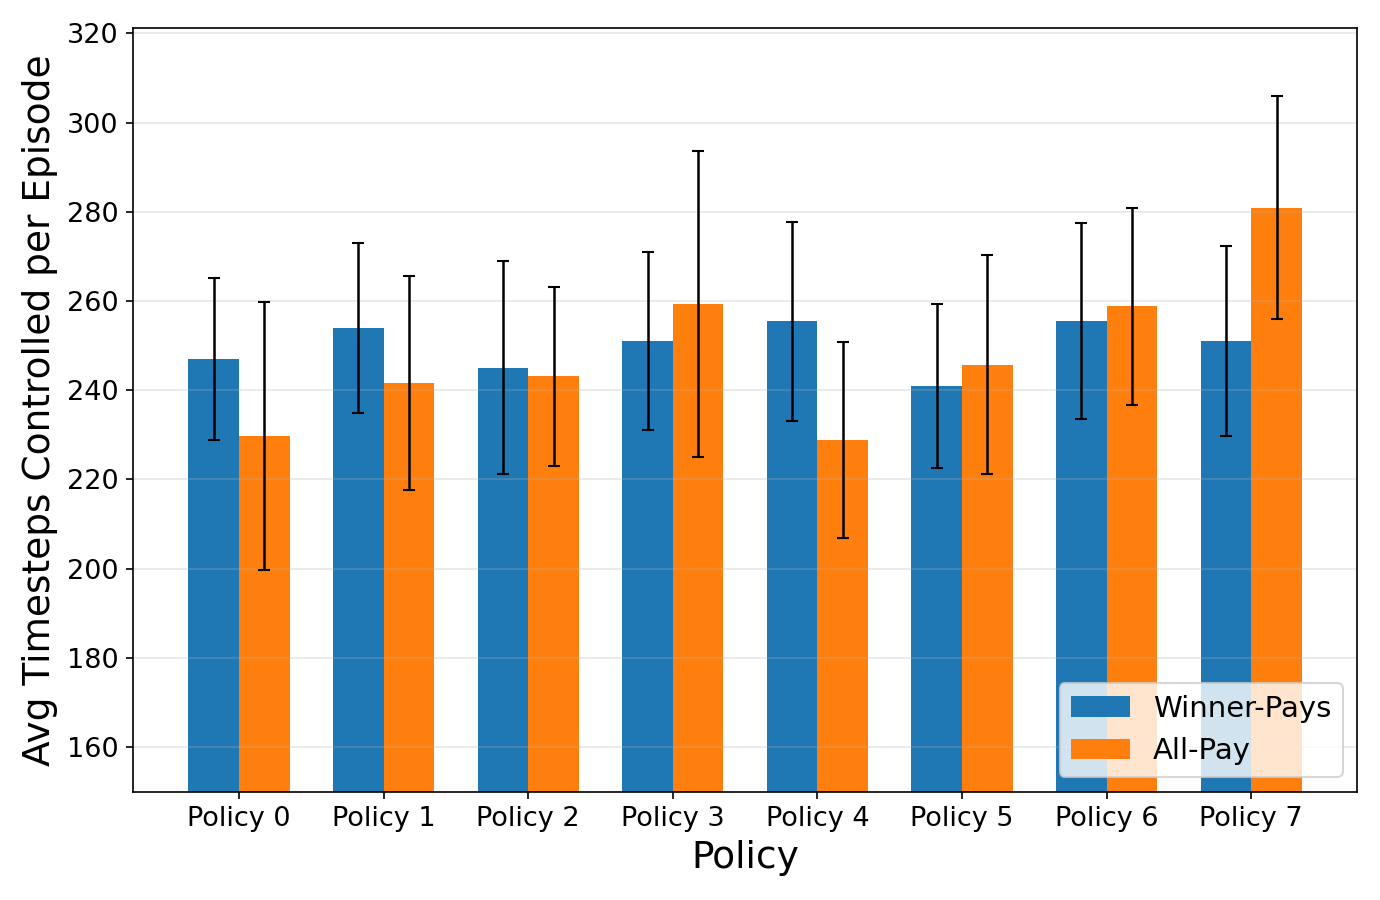
\includegraphics[width=\textwidth]{img/bidding_mechanisms_control_timesteps.png}
        \caption{Cat Feeder.}
        \label{fig:dyntar-control-dist}
    \end{subfigure}
    \hfill
    \begin{subfigure}[t]{0.25\textwidth}
        \centering
        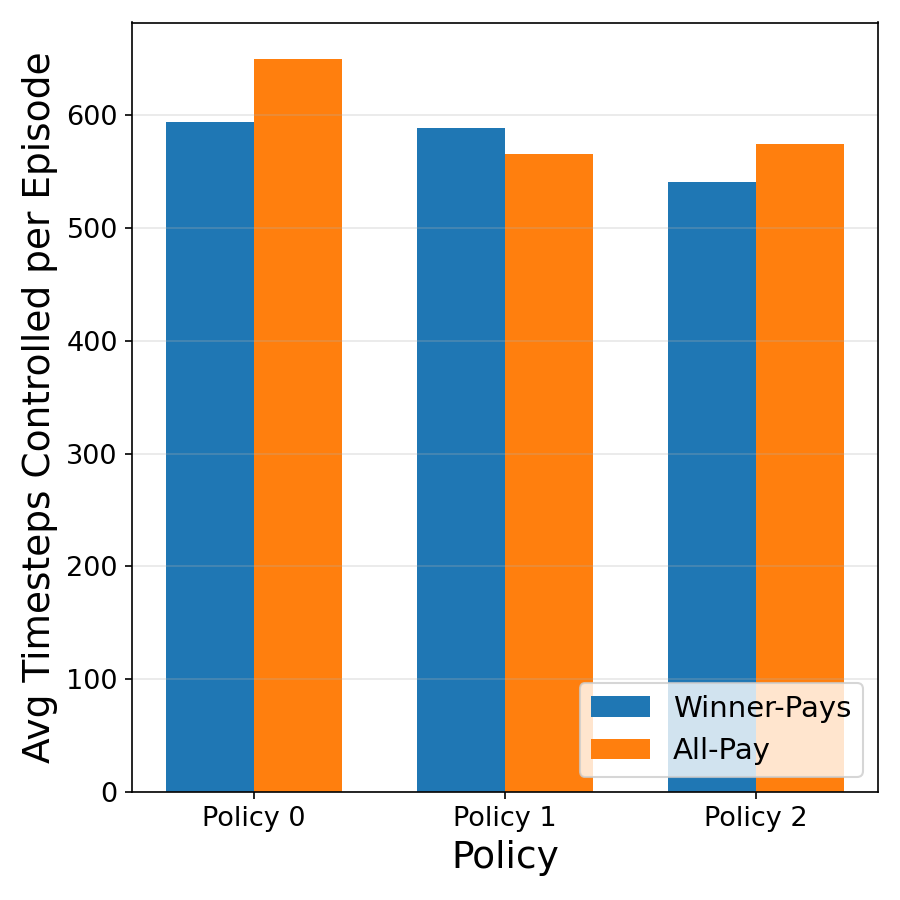
\includegraphics[width=\textwidth]{img/assault_bidding_mechanisms_control_timesteps.png}
        \caption{Atari Assault.}
        \label{fig:assault-control-dist}
    \end{subfigure}
    \hfill
    \begin{subfigure}[t]{0.25\textwidth}
        \centering
        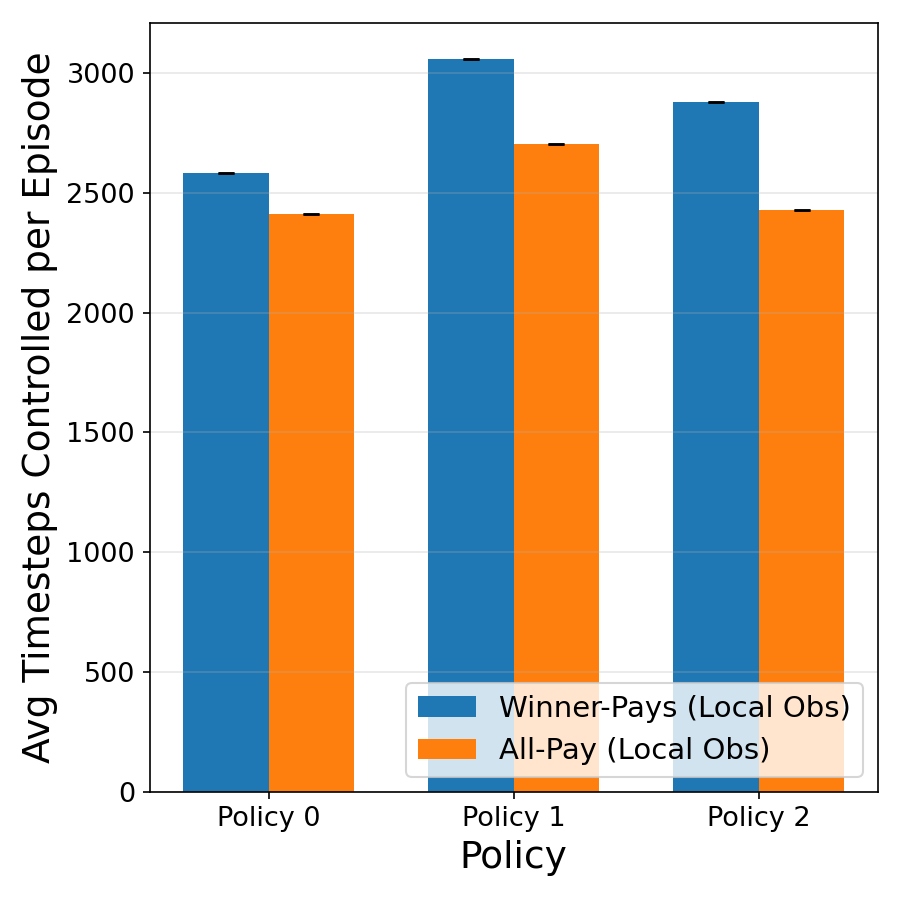
\includegraphics[width=\textwidth]{img/airraid_bidding_mechanisms_control_timesteps.png}
        \caption{Atari Air-Raid.}
        \label{fig:airraid-control-dist}
    \end{subfigure}
    \caption{Control distributions across environments and methods. The control distribution is the number of timesteps controlled by each policy.}
    \label{fig:control-dist-appendix}
\end{figure}

\begin{figure}[h]
    \centering
    \begin{subfigure}[b]{0.3\textwidth}
        \centering
        
\includegraphics[width=\textwidth]{img/gridworld_action_window_bar_chart.png}
        \caption{Cat Feeder.}
    \end{subfigure}
    % \hfill
    \begin{subfigure}[b]{0.3\textwidth}
        \centering
        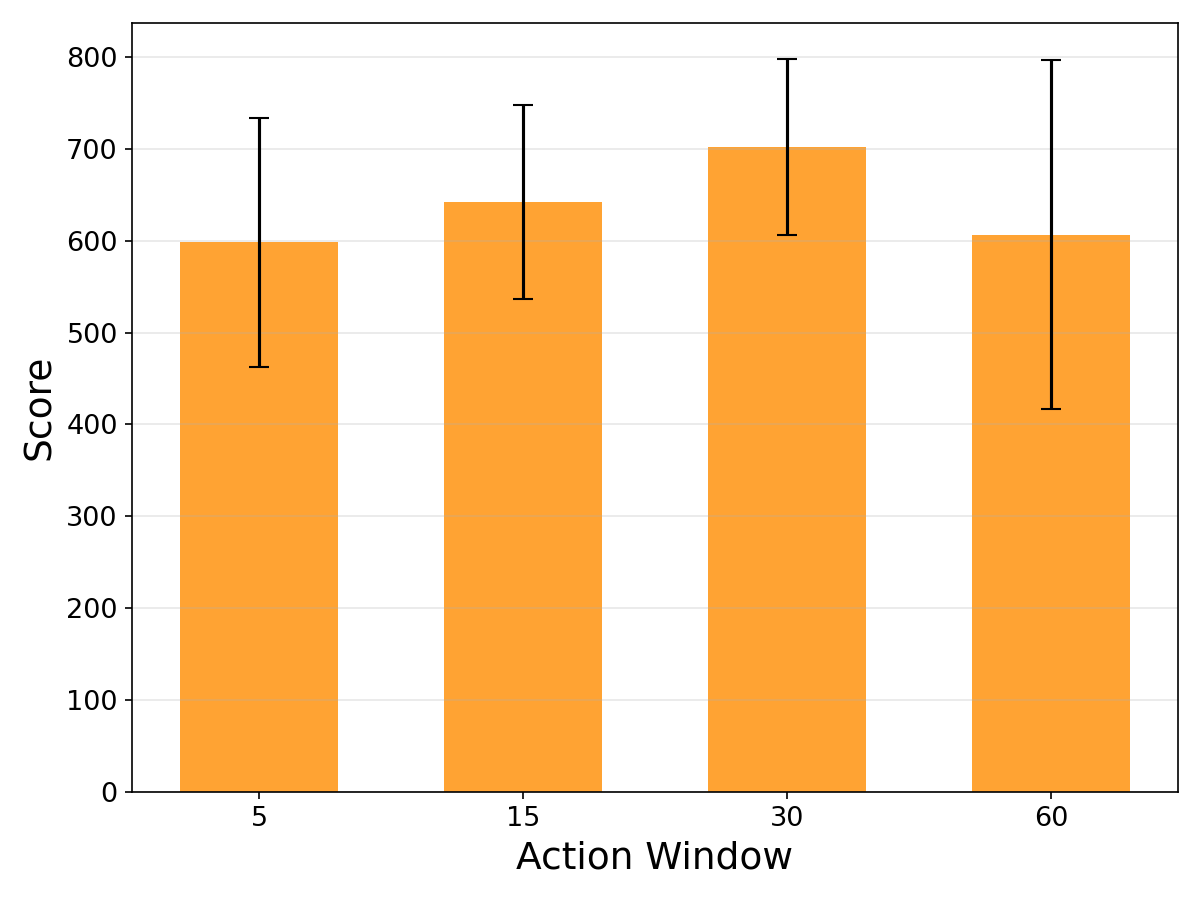
\includegraphics[width=\textwidth]{img/assault_action_window_bar_chart.png}
        \caption{Atari Assault.}
    \end{subfigure}
    \caption{Effect of the action-window size on performance.}
    \label{fig:action-window}
\end{figure}

\Cref{fig:action-window} studies the action-window size in the Cat Feeder and Atari Assault environments.
Smaller windows cause excessive switching between policies, while larger windows prevent sufficient switching to serve all objectives.
The best performance occurs at an intermediate action-window size.
